\documentclass[preprint,12pt]{elsarticle}

\usepackage[margin=1in]{geometry}
\usepackage{graphicx}
\usepackage{booktabs}
\usepackage{array}
\usepackage{caption}
\usepackage{subcaption}
\usepackage{siunitx}
\usepackage{setspace}
\usepackage{microtype}


% --- Numbering as S1, S2, ... ---
\renewcommand{\thefigure}{S\arabic{figure}}
\renewcommand{\thetable}{S\arabic{table}}
\renewcommand{\theequation}{S\arabic{equation}}

\onehalfspacing


\begin{document}

\begin{frontmatter}

%---------------- Title block ----------------
\title{\textbf{Supporting Information}\\[4pt]
\large Developing and Validating a High-Throughput Robotic System for the Accelerated Development of Porous Membranes}

\author[1]{Hongchen Wang}
\author[2]{Sima Zeinali Danalou}
\author[2]{Jiahao Zhu}
\author[2]{Kenneth Sulimro}
\author[3]{Chaewon Lim}
\author[4]{Smita Basak}
\author[1]{Aim\'ee Tai}
\author[4]{Usan Siriwardana}
\author[1]{Jason Hattrick-Simpers \corref{cor1}}
\author[2]{Jay Werber \corref{cor1}}

%% Author affiliation
\affiliation[1]{organization={Department of Materials Science and Engineering, University of Toronto},
            addressline={27 King's College Cir}, 
            city={Toronto},
            postcode={M5S 1A1}, 
            state={ON},
            country={Canada}}
\affiliation[2]{organization={Department of Chemical Engineering, University of Toronto},
            addressline={27 King's College Cir}, 
            city={Toronto},
            postcode={M5S 1A1}, 
            state={ON},
            country={Canada}}
\affiliation[3]{organization={Department of Engineering Science, University of Toronto},
            addressline={27 King's College Cir}, 
            city={Toronto},
            postcode={M5S 1A1}, 
            state={ON},
            country={Canada}}
\affiliation[4]{organization={Department of Mechanical Engineering, University of Waterloo},
            addressline={200 University Ave W}, 
            city={Waterloo},
            postcode={N2L 3G1}, 
            state={ON},
            country={Canada}}

\cortext[cor1]{Corresponding authors: jason.hattrick-simpers@utoronto.ca; jay.werber@utoronto.ca}

\end{frontmatter}
\clearpage

\section{Supplementary SEM Images of Nitrogen-Treated PSf Membranes}

\begin{figure*}[ht]
\centering
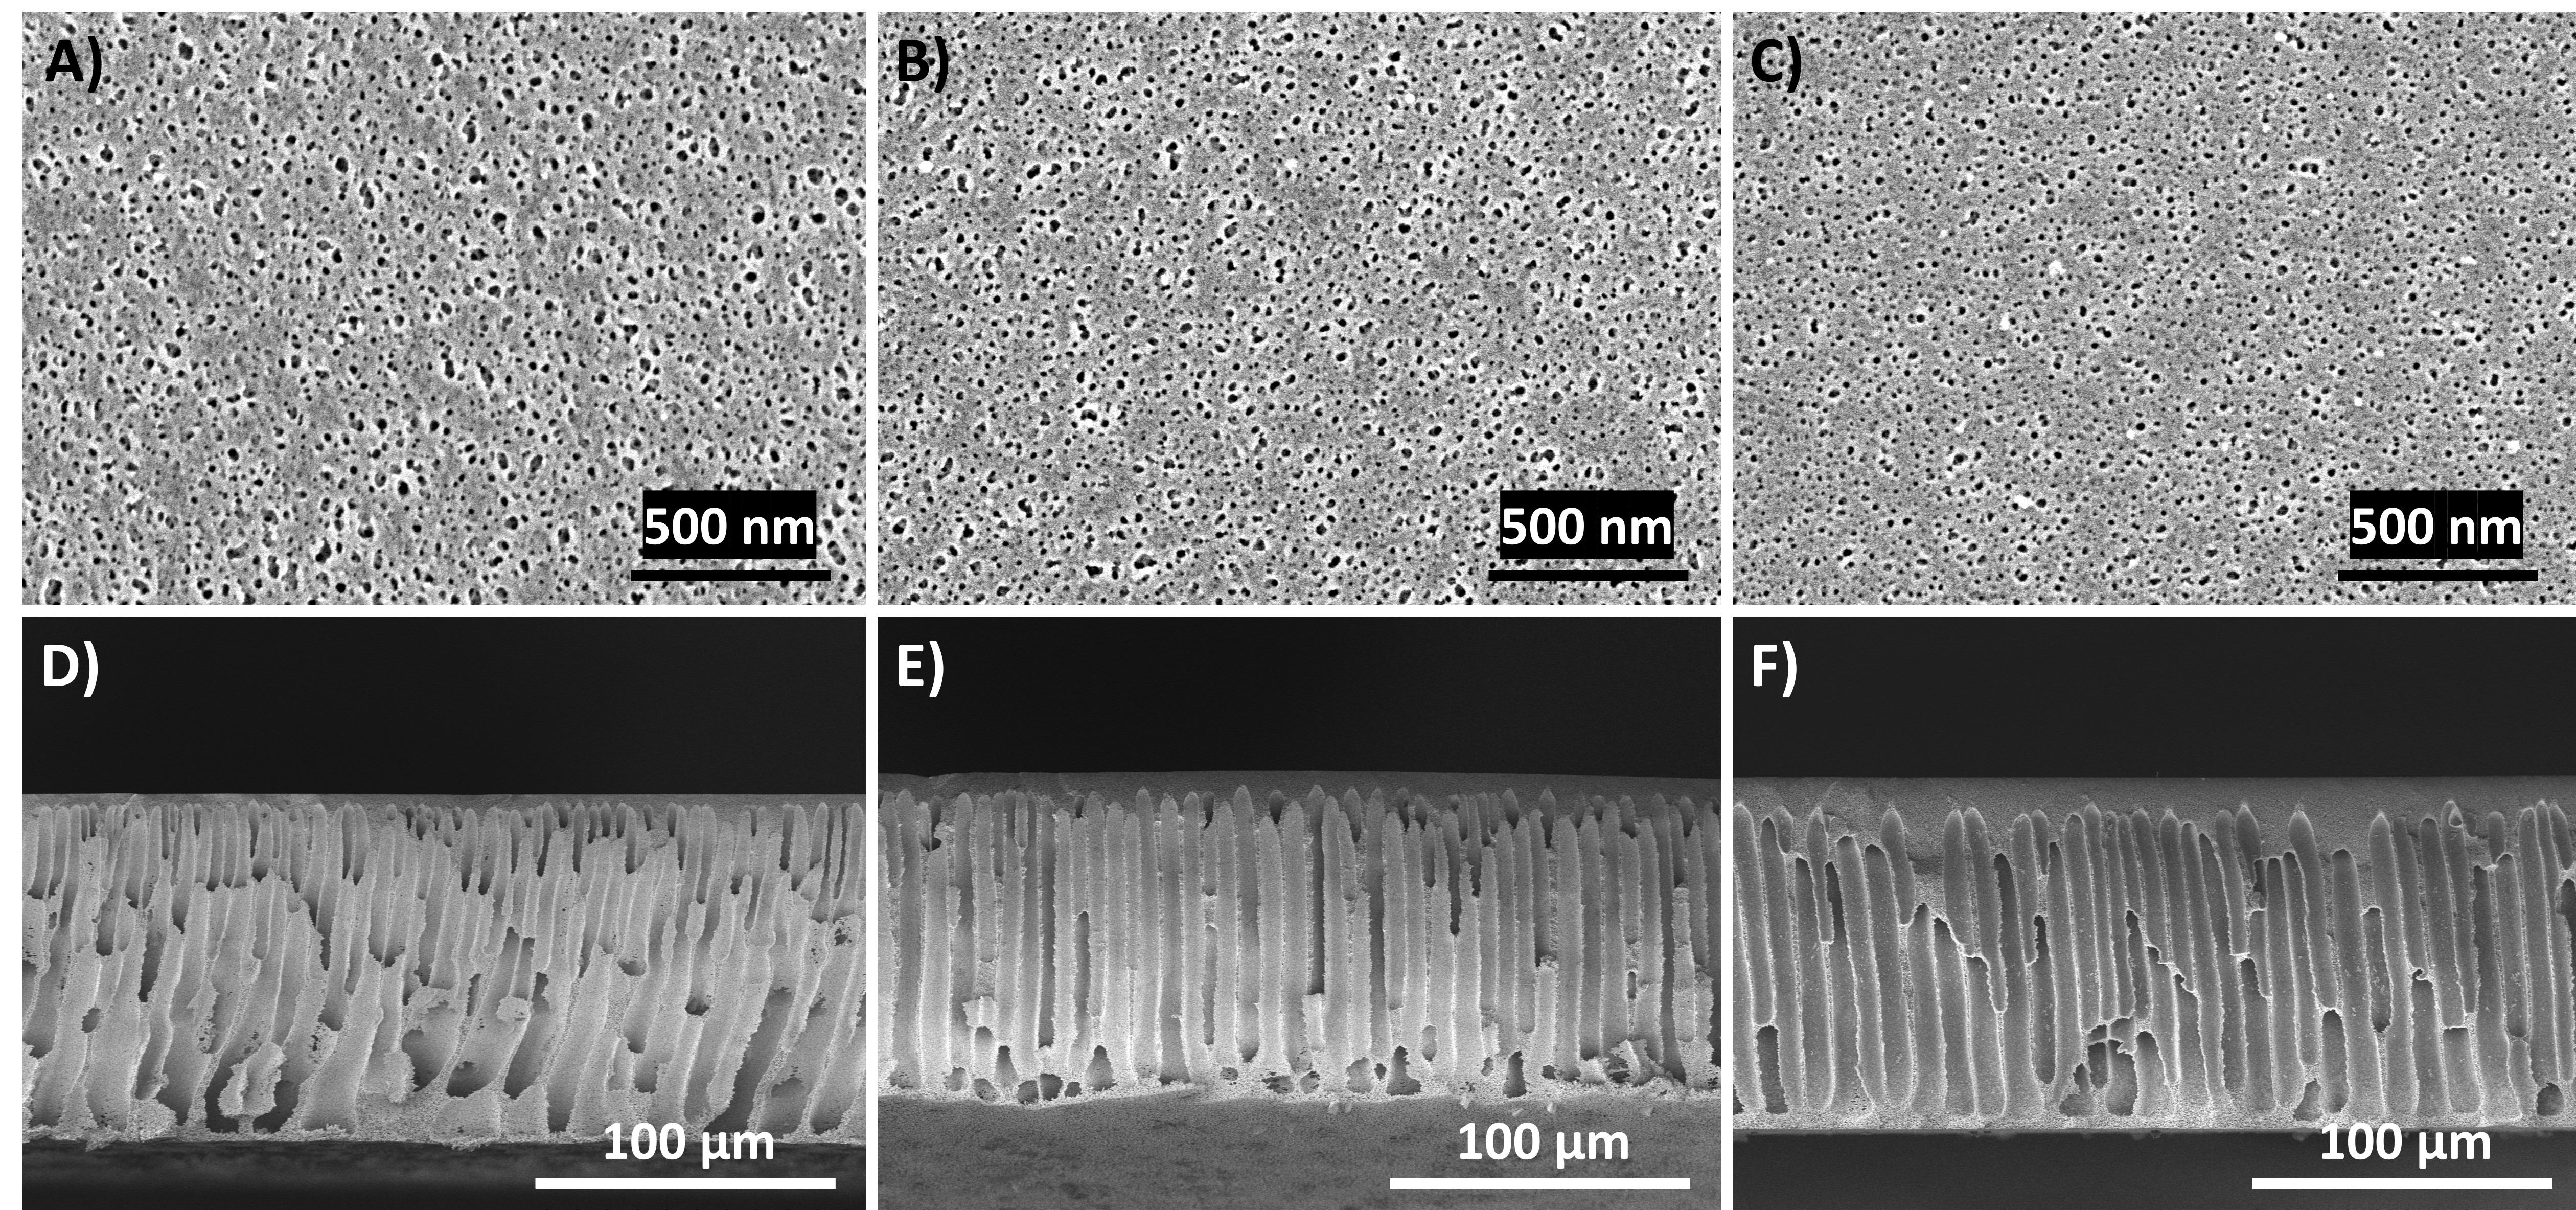
\includegraphics[width=0.9\linewidth]{PSD_SI.jpg}
\caption{SEM and processed binary images of nitrogen‑treated PSf membranes fabricated with polymer concentrations of 10 wt\% (A, D, G, J), 12 wt\% (B, E, H, K), and 15 wt\% (C, F, I, L). (A–C) pristine cross‑sections; (D–F) pristine top views; (G–I) binary images of the coated top views; (J–L) binary images after correcting for sputter‑coating‑induced pore narrowing. All samples were produced on the fully automated, nitrogen‑assisted casting platform.}
\label{PSD_SI.jpg}
\end{figure*}
\clearpage

\section{Commercial Equipment Used in the Automated Platform}
The automated membrane fabrication and testing platform was constructed using the following commercially available tools shown in Table \ref{list of machines}

\begin{table}[!ht]
\centering
\begin{tabular}{ll}
\hline
\textbf{Equipment} & \textbf{Function} \\
\hline
Opentrons OT-2 & Solution preparation and dispensing \\
Opentrons Temperature Module & Solution heating \\
Ufactory xArm7 & Blade casting and sample pick-and-place \\
TestResources 140 & Mechanical characterization (compression testing) \\
IKA RC 2 Lite & Coagulation bath temperature control \\
\hline
\end{tabular}
\caption{Commercial tools used in the automated membrane fabrication and testing platform.}
\label{list of machines}
\end{table}


\section{Optimization of Opentrons OT-2 Pipetting Parameters for High-Viscosity Solutions}
\begin{figure}[h]
\centering
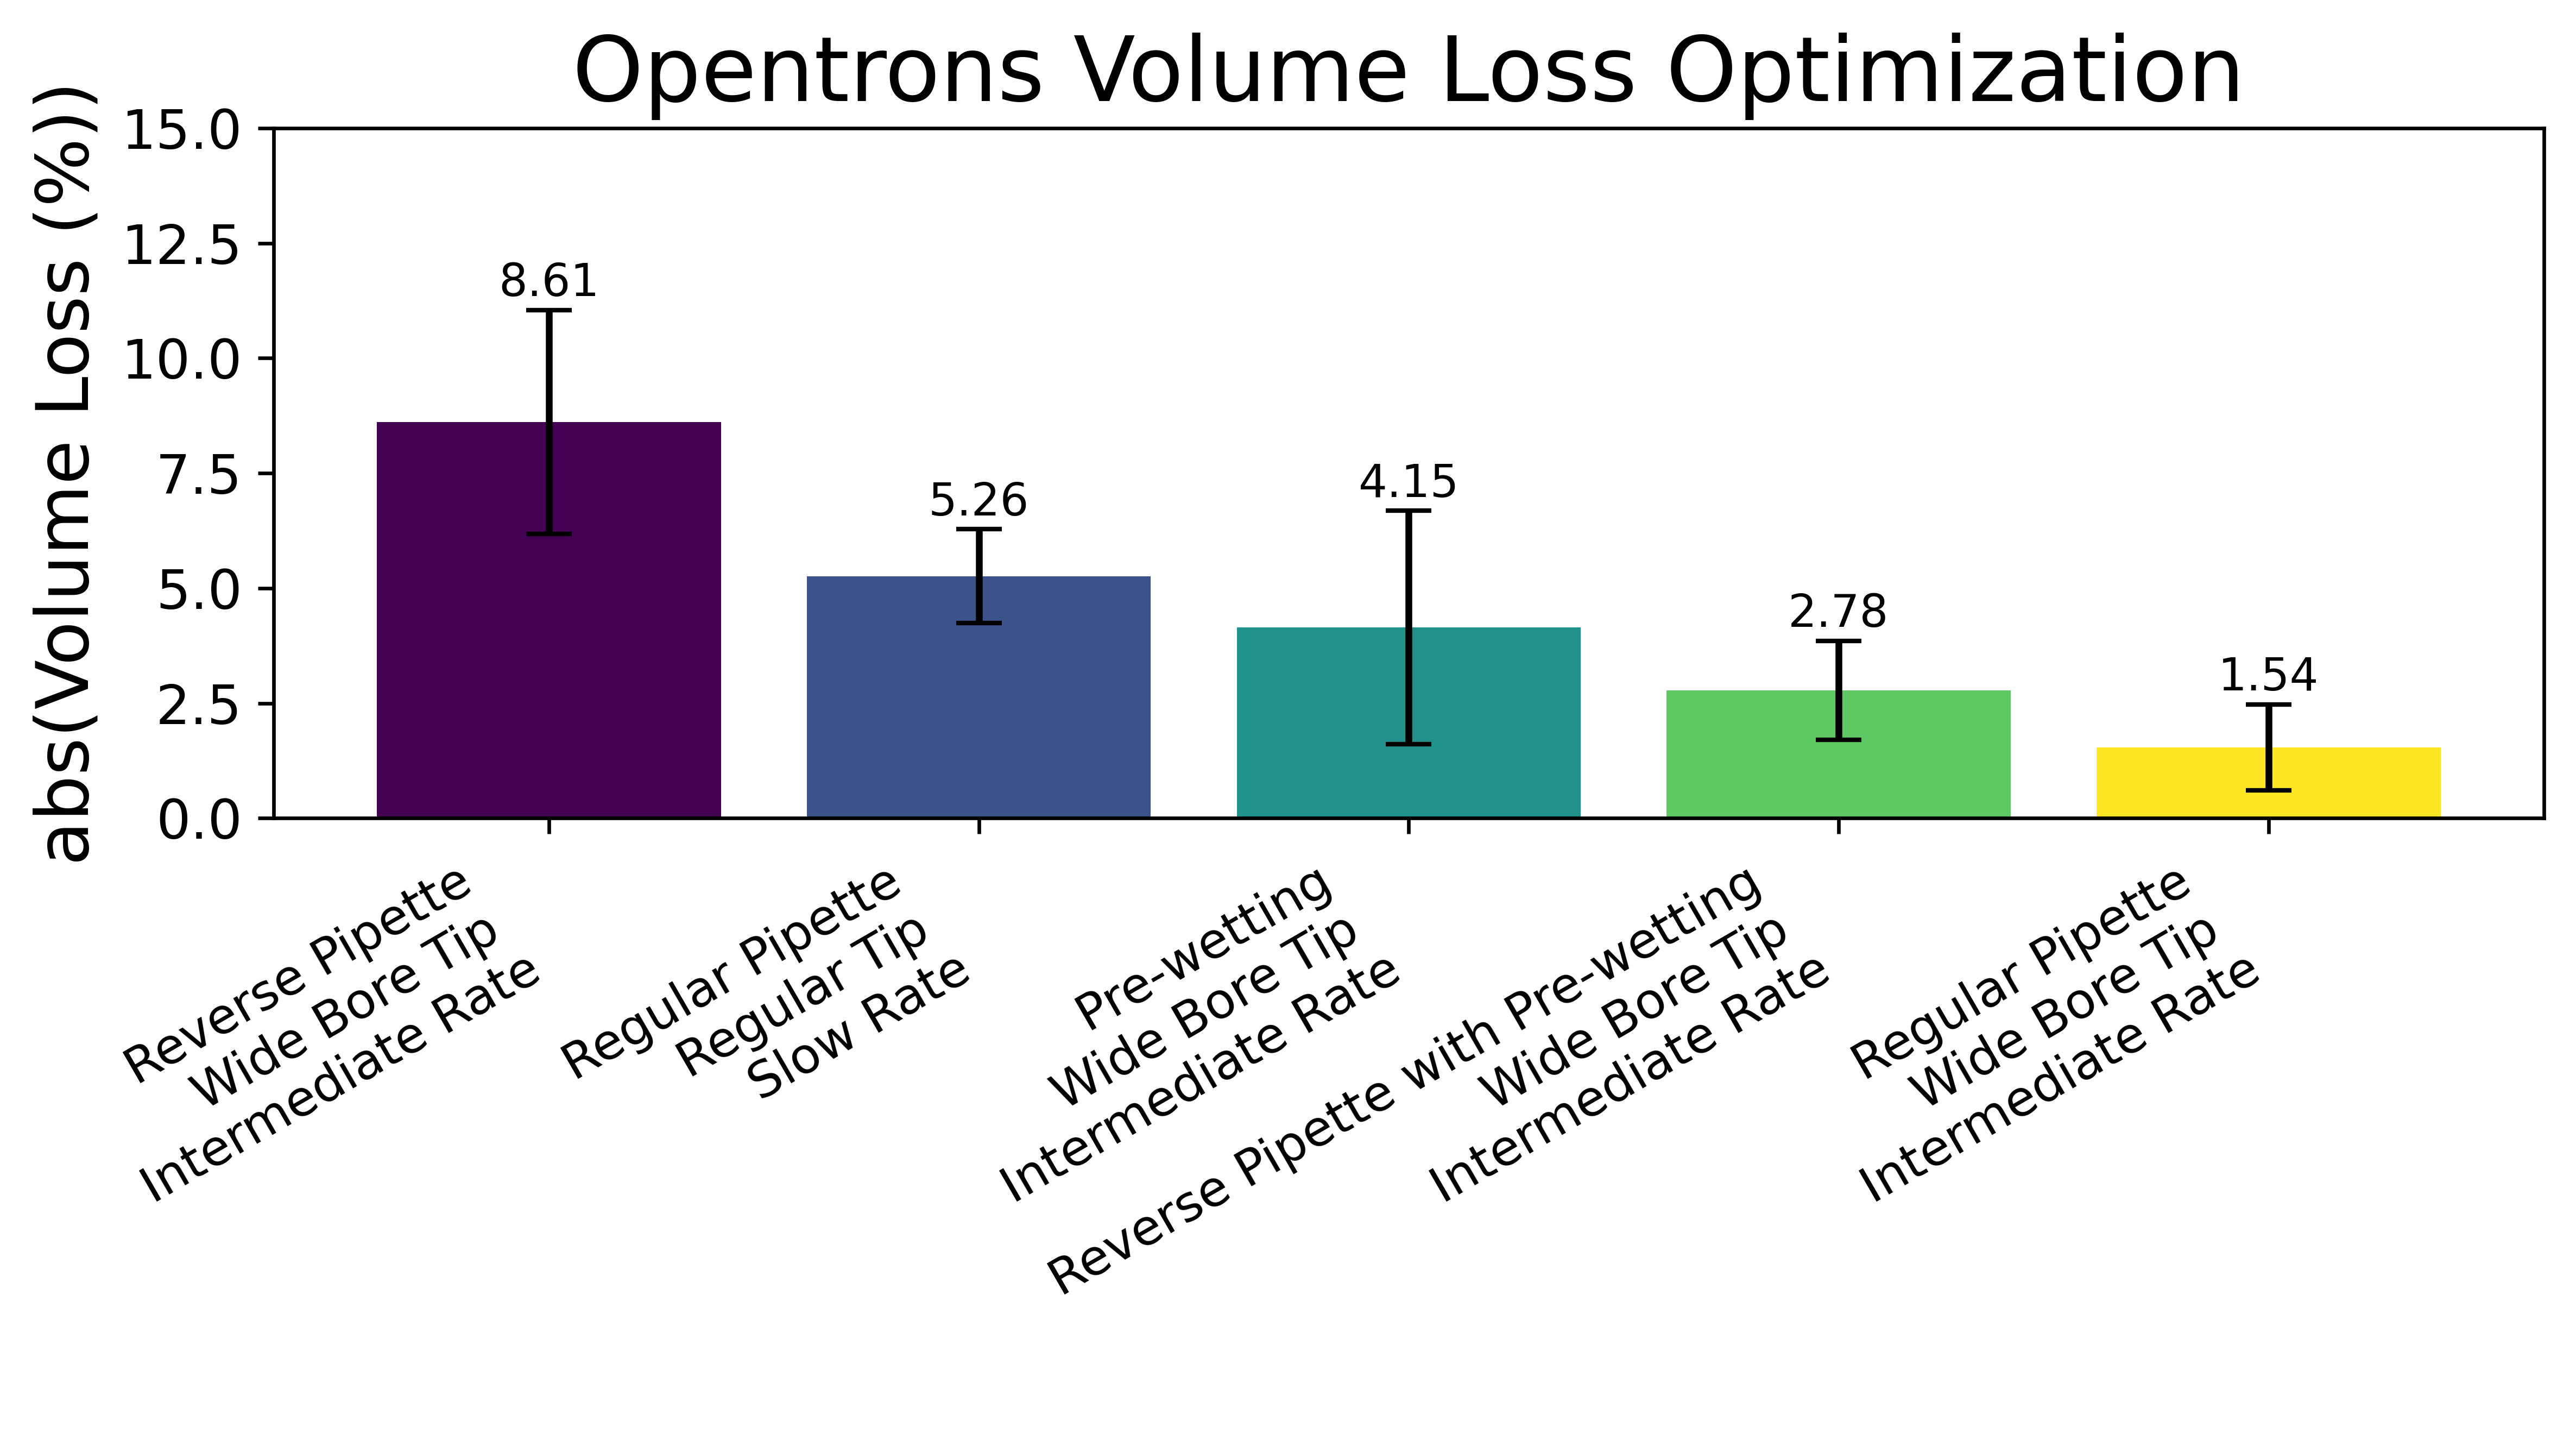
\includegraphics[width=0.6\linewidth]{opentrons.png}
\caption{Effect of pipetting strategies on volume loss during automated liquid handling of a high-viscosity polymer solution using the Opentrons OT-2. Various tip types, pipetting modes (regular vs. reverse), and pre-wetting conditions were evaluated. Regular pipetting with wide bore tips at intermediate speed resulted in the lowest volume loss.}
\label{opentrons.png}
\end{figure}
\clearpage


\section{Optimized Opentrons OT-2 Pipetting Parameters}
\begin{table}[htbp]
\centering
\caption{Opentrons pipette parameters for viscous (i.e., stock solution) vs.\ non‑viscous (i.e., solvent) liquids.}
\label{tab:opentrons_liquid_specific}
\begin{tabular}{lcc}
\hline
\textbf{Parameter} & \textbf{Viscous} & \textbf{Non‑viscous} \\
\hline
Aspiration rate                 & 3          & 200  \\
Aspiration delay                & 30         & 0.1  \\
Aspiration withdraw rate        & 1          & 10   \\
Dispense rate                   & 3          & 400  \\
Dispense delay                  & 30         & 0.1  \\
Dispense air delay              & 0.1        & 0    \\
Dispense withdraw rate          & 1          & 10   \\
Blow‑out rate                   & 8          & 1000 \\
Mix aspiration rate             & 15         & 200  \\
Mix dispense rate               & 15         & 400  \\
\hline
\end{tabular}
\end{table}

%-------------------------------------------------
% Table 2 – Parameters common to both liquid types
\begin{table}[htbp]
\centering
\caption{Settings and parameters for solution mixing.}
\label{tab:opentrons_common_params}
\begin{tabular}{lc}
\hline
\textbf{Parameter} & \textbf{Value} \\
\hline
Mix delay     & 0.1 \\
Mix times     & 10  \\
Mix volume    & 820 \\
Air‑gap volume & 10  \\
\hline
\end{tabular}
\end{table}


\section{Demonstration Video of the Automated System}
A video demonstrating the operation of the automated membrane fabrication and testing system is available at the following link: \texttt{https://youtu.be/PrFT4oi4K5g?si=0IpMpfhhs\_fAqntw}

\end{document}
